%%%%%%%%%%%%%%%%%%%%%%%%%%%%%%%%%%%%%%%%%
% fphw Assignment
% LaTeX Template
% Version 1.0 (27/04/2019)
%
% This template originates from:
% https://www.LaTeXTemplates.com
%
% Authors:
% Class by Felipe Portales-Oliva (f.portales.oliva@gmail.com) with template 
% content and modifications by Vel (vel@LaTeXTemplates.com)
%
% Template (this file) License:
% CC BY-NC-SA 3.0 (http://creativecommons.org/licenses/by-nc-sa/3.0/)
%
%%%%%%%%%%%%%%%%%%%%%%%%%%%%%%%%%%%%%%%%%

%----------------------------------------------------------------------------------------
%	PACKAGES AND OTHER DOCUMENT CONFIGURATIONS
%----------------------------------------------------------------------------------------

\documentclass[
	12pt,
	%fleqn, % Default font size, values between 10pt-12pt are allowed
	%letterpaper, % Uncomment for US letter paper size
	%spanish, % Uncomment for Spanish
]{fphw}

% Template-specific packages
\usepackage[utf8]{inputenc} % Required for inputting international characters
\usepackage[T1]{fontenc} % Output font encoding for international characters
\usepackage{mathpazo} % Use the Palatino font

\usepackage{graphicx} % Required for including images

\usepackage{booktabs} % Required for better horizontal rules in tables

\usepackage{listings} % Required for insertion of code

\usepackage{enumerate} % To modify the enumerate environment

\usepackage{enumitem}

\usepackage{amsmath}

\usepackage{mathtools,amsthm}

\usepackage{float}

\usepackage{listings}

\usepackage{hyperref}

\usepackage{tikz}

\lstdefinelanguage{R}{
  keywords={if, else, repeat, while, function, for, in, next, break},
  otherkeywords={TRUE, FALSE, NULL, NA, Inf, NaN},
  sensitive=true,
  morecomment=[l]\#,
  morestring=[b]",
}

\newcommand{\E}{\mathbb{E}}
\newcommand{\Var}{\operatorname{Var}}
\newcommand{\R}{\mathbb{R}}
\newcommand{\norm}[1]{\left\lVert #1 \right\rVert}


%----------------------------------------------------------------------------------------
%	ASSIGNMENT INFORMATION
%----------------------------------------------------------------------------------------

\title{Homework \#11} % Assignment title

\author{Shizhe Zhang} % Student name

\date{\today} % Due date

\institute{University of California, Berkeley \\ Department of Statistics} % Institute or school name

\class{EECS 227AT} % Course or class name

\professor{Gireeja Ranade} % Professor or teacher in charge of the assignment

%----------------------------------------------------------------------------------------

\begin{document}

\maketitle % Output the assignment title, created automatically using the information in the custom commands above

%----------------------------------------------------------------------------------------
%	ASSIGNMENT CONTENT
%----------------------------------------------------------------------------------------

\section*{Problem 1. Linear Programming}

Express the following problem as an LP.

\[
\min_{x \in \mathbb{R}^k} \sum_{i=1}^{k} |x_i| \tag{1}
\]

\[
\text{s.t. } A x = b \tag{2}
\]

\subsection*{Answer}

Introduce auxiliary variables $t_i \ge 0$ such that $t_i \ge |x_i|$.
This can be written using linear inequalities:

\[
x_i \le t_i, \quad -x_i \le t_i, \quad i=1,\dots,k.
\]

Then the problem becomes the following linear program:

\[
\min_{x,t} \sum_{i=1}^{k} t_i
\]

\[
\text{s.t. } Ax = b
\]

\[
x_i - t_i \le 0, \quad i=1,\dots,k
\]

\[
-x_i - t_i \le 0, \quad i=1,\dots,k
\]

\[
t_i \ge 0, \quad i=1,\dots,k.
\]

At optimality, minimizing $\sum_i t_i$ ensures $t_i = |x_i|$, so this LP is equivalent to the original problem.





%----------------------------------------------------------------------------------------
\newpage
\section*{Problem 2. Fun with Hyperplanes}

In this problem we work with hyperplanes, which are key components of linear programming as well as future
topics such as support vector machines.

(a) Sketch the hyperplane \(H := \{\vec x \in \mathbb{R}^2 \mid [1\quad 1]\vec x = 2\}\).

(b) Let \(c \in \mathbb{R}^n\) be nonzero, and let \(H := \{x \in \mathbb{R}^n \mid c^\top x = 0\}\).
Show that \(H\) is a linear subspace of \(\mathbb{R}^n\). What is \(\dim(H)\)?

(c) Let \(c \in \mathbb{R}^n\) be nonzero, and let \(H := \{x \in \mathbb{R}^n \mid c^\top x = 0\}\).
Suppose \(x^\star \in \mathbb{R}^n\) is on one side of the hyperplane, i.e., \(c^\top x^\star > 0\).
Give any vector which is on the other side of the hyperplane but not on the hyperplane itself.

(d) Let \(c \in \mathbb{R}^n\) be nonzero, and let \(x_0 \in \mathbb{R}^n\) be arbitrary.
Let \(H := \{x \in \mathbb{R}^n \mid c^\top (x - x_0) = 0\}\).
Suppose \(x^\star \in \mathbb{R}^n\) is on one side of the hyperplane.
Give any vector which is on the other side of the hyperplane but not on the hyperplane itself.

(e) Let \(x_0 \in \mathbb{R}^n\) be arbitrary. For a vector \(c \in \mathbb{R}^n\), let
\(H(c) := \{x \in \mathbb{R}^n \mid c^\top (x - x_0) = 0\}\).
Show that \(0 \in H(c)\) for every \(c \in \mathbb{R}^n\) if and only if \(x_0 = 0\).

\subsection*{Answer}

(a)
\begin{center}
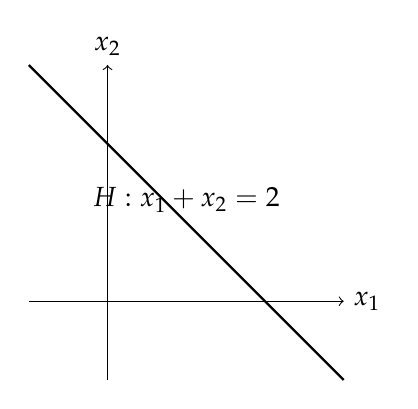
\begin{tikzpicture}
    \draw[->] (-1,0) -- (3,0) node[right] {$x_1$};
    \draw[->] (0,-1) -- (0,3) node[above] {$x_2$};
    \draw[thick] (-1,3) -- (3,-1) node[pos=0.5, above] {$H: x_1 + x_2 = 2$};
\end{tikzpicture}
\end{center}

(b) Let
\[
H = \{x \in \mathbb{R}^n \mid c^\top x = 0\},
\]
where $c \neq 0$.

To show $H$ is a linear subspace, verify the three properties:

\textbf{Contains zero:}
\[
c^\top 0 = 0
\]
so $0 \in H$.

\textbf{Closed under addition:}  
If $x,y \in H$, then
\[
c^\top x = 0, \quad c^\top y = 0.
\]
Thus
\[
c^\top (x+y) = c^\top x + c^\top y = 0,
\]
so $x+y \in H$.

\textbf{Closed under scalar multiplication:}  
For $\alpha \in \mathbb{R}$ and $x \in H$,
\[
c^\top (\alpha x) = \alpha c^\top x = 0,
\]
so $\alpha x \in H$.

Thus $H$ is a linear subspace of $\mathbb{R}^n$.

Since the constraint $c^\top x = 0$ removes one degree of freedom and $c \neq 0$,

\[
\dim(H) = n-1.
\]

\bigskip

(c) Suppose $x^\star$ satisfies
\[
c^\top x^\star > 0.
\]
Then the vector
\[
-x^\star
\]
satisfies
\[
c^\top (-x^\star) = -c^\top x^\star < 0.
\]

Thus $-x^\star$ lies on the opposite side of the hyperplane and is not on the hyperplane.

\bigskip

(d) Let
\[
H = \{x \in \mathbb{R}^n \mid c^\top (x-x_0)=0\}.
\]

If $x^\star$ is on one side, then
\[
c^\top (x^\star - x_0) > 0.
\]

Consider
\[
x = 2x_0 - x^\star .
\]

Then
\[
x - x_0 = x_0 - x^\star = -(x^\star - x_0),
\]

so

\[
c^\top (x-x_0) = -c^\top (x^\star - x_0) < 0.
\]

Thus $x$ lies on the opposite side of the hyperplane and is not on it.

\bigskip

(e) Let
\[
H(c) = \{x \in \mathbb{R}^n \mid c^\top (x-x_0)=0\}.
\]

Suppose $0 \in H(c)$ for every $c \in \mathbb{R}^n$. Then

\[
c^\top (0-x_0) = 0
\]

for all $c$, which implies

\[
c^\top x_0 = 0
\]

This is only possible if

\[
x_0 = 0.
\]

Conversely, if $x_0=0$, then

\[
c^\top (0-x_0) = 0
\]

for all $c$, so $0 \in H(c)$ for every $c$.

Thus

\[
0 \in H(c) \text{ for every } c \iff x_0 = 0.
\]



%----------------------------------------------------------------------------------------
\newpage
\section*{Problem 3. LP at Boundary}

Consider the LP:

\[
\min_{x \in \mathbb{R}^n} c^\top x \tag{3}
\]

\[
\text{s.t. } Ax \le b \tag{4}
\]

Here we have non-zero \(c \in \mathbb{R}^n\), \(x \in \mathbb{R}^n\), \(A \in \mathbb{R}^{m\times n}\), and \(b \in \mathbb{R}^m\).
The feasible set forms a polyhedron

\[
P = \{x \in \mathbb{R}^n \mid a_i^\top x - b_i \le 0,\ 1 \le i \le n\} \tag{5}
\]

\[
= \bigcap_{i=1}^{m} \{x \in \mathbb{R}^n \mid a_i^\top x - b_i \le 0\}. \tag{6}
\]

In the second line, \(P\) is defined as the intersection of half-spaces.
When this set is bounded, it is often referred to as a polytope instead.

In this problem we will prove facts about linear programs, including the crucial fact that the solution to an LP
exists at the boundary of a polytope.

(a) First, consider the case where we have an unbounded polyhedron.
For any such \(P\), assume there exists some \(x_0, v \in \mathbb{R}^n\) with \(x_0 \ne v\) such that

\[
L := \{x_0 + \alpha v \mid \alpha \in [0,\infty)\} \subset P .
\]

This is saying that there exists a line segment, unbounded on one side, that is contained within \(P\).
Show that if \(c^\top v < 0\), then \(p^\star = -\infty\).

(b) Now, suppose our feasible set is defined by a bounded polytope (i.e. a polytope that contains its boundary).
We say a point belongs to the interior of \(P\) (i.e. \(x_0 \in \text{Int}(P)\)) if there exists some ball of radius
\(\epsilon > 0\) such that

\[
B := \{y \in \mathbb{R}^n \mid \|y - x_0\|_2 \le \epsilon\} \subset P .
\]

Show that the optimal point for the LP cannot be obtained in the interior of \(P\) and must be obtained on the
boundary (that is, when for some \(1 \le i \le n\), \(a_i^\top x - b_i = 0\)).
For this, consider a proof by contradiction. Show that for any \(x_0\) on the interior, there exists another point

\[
x_1 := x_0 - \epsilon \frac{c}{\|c\|_2} \tag{7}
\]

such that \(x_1 \in P\) and \(c^\top x_1 < c^\top x_0\).

\subsection*{Answer}

(a) Suppose the polyhedron $P$ is unbounded and there exist $x_0, v \in \mathbb{R}^n$ such that
\[
L := \{x_0 + \alpha v \mid \alpha \in [0,\infty)\} \subset P.
\]

Then for any $\alpha \ge 0$, the point $x(\alpha) = x_0 + \alpha v$ is feasible. The objective value is

\[
c^\top x(\alpha) = c^\top (x_0 + \alpha v)
= c^\top x_0 + \alpha c^\top v.
\]

If $c^\top v < 0$, then as $\alpha \to \infty$,

\[
c^\top x(\alpha) \to -\infty.
\]

Thus the objective can be made arbitrarily small while remaining feasible, so the optimal value is

\[
p^\star = -\infty.
\]

\bigskip

(b) Suppose $P$ is a bounded polytope and assume for contradiction that the optimal solution $x_0$ lies in the interior of $P$.

By definition of interior, there exists $\epsilon > 0$ such that the ball
\[
B = \{y \in \mathbb{R}^n \mid \|y - x_0\|_2 \le \epsilon\}
\]
is contained in $P$.

Consider the point

\[
x_1 = x_0 - \epsilon \frac{c}{\|c\|_2}.
\]

\[
\|x_1 - x_0\|_2
=
\left\|\epsilon \frac{c}{\|c\|_2}\right\|_2
=
\epsilon.
\]

Thus $x_1 \in B$, and since $B \subset P$, we have $x_1 \in P$.

Now compare objective values:

\[
c^\top x_1
=
c^\top \left(x_0 - \epsilon \frac{c}{\|c\|_2}\right)
=
c^\top x_0 - \epsilon \frac{c^\top c}{\|c\|_2}.
\]

Since $c^\top c = \|c\|_2^2$, this becomes

\[
c^\top x_1
=
c^\top x_0 - \epsilon \|c\|_2.
\]

Because $\epsilon > 0$ and $\|c\|_2 > 0$,

\[
c^\top x_1 < c^\top x_0.
\]

Thus $x_1$ is feasible and has a strictly smaller objective value than $x_0$, contradicting the assumption that $x_0$ is optimal.

Therefore, the optimal solution cannot lie in the interior of $P$. It must occur on the boundary, i.e., for some constraint

\[
a_i^\top x - b_i = 0.
\]




%----------------------------------------------------------------------------------------
\newpage
\section*{Problem 4. Linear Programs}

Consider the following linear program:

\[
\max_{x_1,x_2 \in \mathbb{R}} 2x_1 + 3x_2 \tag{8}
\]

\[
x_1 + 2x_2 \le 8 \tag{9}
\]

\[
x_1 - x_2 \le 2 \tag{10}
\]

\[
x_2 + x_1 \ge 2 \tag{11}
\]

\[
x_1 \ge 0 \tag{12}
\]

\[
x_2 \ge 0 \tag{13}
\]

(a) Sketch the feasible region of the linear program as well as the 5-, 10-, and 15-level sets of the objective
function.

HINT: Recall that for \(f : \mathbb{R}^n \to \mathbb{R}\) and \(\alpha \in \mathbb{R}\), the \(\alpha\)-level set of \(f\)
is defined as \(\{x \in \mathbb{R}^n : f(x) = \alpha\}\).

(b) Express the linear program in the following form:

\[
\max_{x \in \mathbb{R}^n} c^\top x \tag{14}
\]

\[
\text{s.t. } Ax \le b \tag{15}
\]

Specify the values of \(x\), \(c\), \(A\), and \(b\).

(c) Express the linear program in the following form:

\[
\min_{y \in \mathbb{R}^n} c^\top y \tag{16}
\]

\[
\text{s.t. } Ay = b \tag{17}
\]

\[
y \ge 0 \tag{18}
\]

Specify the values of \(y\), \(c\), \(A\), and \(b\).

HINT: Consider adding additional slack variables to the optimization problem.

(d) List the extreme points or vertices of the feasible region of the linear program given by equations (8)–(13).

(e) Find the optimal value \(p^\star\) and the optimal point
\(x^\star = (x_1^\star, x_2^\star)\) of the linear program given by equations (8)–(13).

HINT: Recall that for a linear program with a bounded feasible region, at least one optimal point is a vertex
of the feasible region.

\subsection*{Answer}
(a) 

The level sets of the objective function

\[
2x_1 + 3x_2 = \alpha
\]

\begin{center}
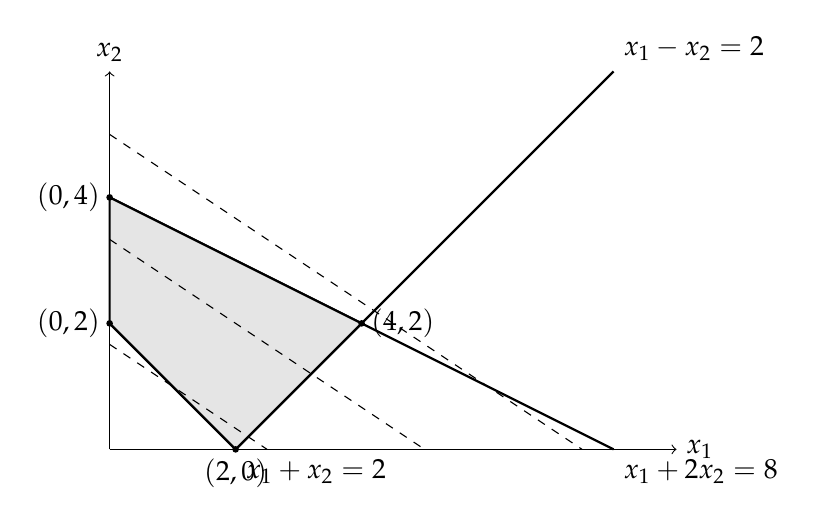
\begin{tikzpicture}[scale=0.8]

% axes
\draw[->] (0,0) -- (9,0) node[right] {$x_1$};
\draw[->] (0,0) -- (0,6) node[above] {$x_2$};

% constraint lines
\draw[thick] (0,4) -- (8,0) node[below right] {$x_1+2x_2=8$};
\draw[thick] (2,0) -- (8,6) node[above right] {$x_1-x_2=2$};
\draw[thick] (0,2) -- (2,0) node[below right] {$x_1+x_2=2$};

% feasible region (exact polygon)
\fill[gray!20] (0,2) -- (2,0) -- (4,2) -- (0,4) -- cycle;
\draw[thick] (0,2) -- (2,0) -- (4,2) -- (0,4) -- cycle;

% level sets: 2x_1 + 3x_2 = alpha
\draw[dashed] (0,5/3) -- (2.5,0) node[below right] {};
\draw[dashed] (0,10/3) -- (5,0) node[below right] {};
\draw[dashed] (0,5) -- (7.5,0) node[below right] {};

% vertices
\fill (0,2) circle (1.5pt) node[left] {$(0,2)$};
\fill (2,0) circle (1.5pt) node[below] {$(2,0)$};
\fill (4,2) circle (1.5pt) node[right] {$(4,2)$};
\fill (0,4) circle (1.5pt) node[left] {$(0,4)$};

\end{tikzpicture}
\end{center}

\bigskip

(b) Write the LP in the form

\[
\max_{x \in \mathbb{R}^2} c^\top x
\]

\[
\text{s.t. } Ax \le b.
\]

We have

\[
x =
\begin{bmatrix}
x_1 \\
x_2
\end{bmatrix},
\qquad
c =
\begin{bmatrix}
2 \\
3
\end{bmatrix}.
\]

The constraints become

\[
A =
\begin{bmatrix}
1 & 2 \\
1 & -1 \\
-1 & -1 \\
-1 & 0 \\
0 & -1
\end{bmatrix},
\qquad
b =
\begin{bmatrix}
8 \\
2 \\
-2 \\
0 \\
0
\end{bmatrix}.
\]

\bigskip

(c) Convert to standard form

\[
\min_{y} c^\top y
\]

\[
Ay = b, \quad y \ge 0.
\]

Introduce slack variables

\[
s_1,s_2,s_3 \ge 0.
\]

Rewrite constraints:

\[
x_1 + 2x_2 + s_1 = 8
\]

\[
x_1 - x_2 + s_2 = 2
\]

\[
x_1 + x_2 - s_3 = 2
\]

Define

\[
y =
\begin{bmatrix}
x_1\\
x_2\\
s_1\\
s_2\\
s_3
\end{bmatrix}.
\]

Objective (convert max to min):

\[
\min -2x_1 -3x_2
\]

so

\[
c =
\begin{bmatrix}
-2\\
-3\\
0\\
0\\
0
\end{bmatrix}.
\]

Matrix form

\[
A =
\begin{bmatrix}
1 & 2 & 1 & 0 & 0 \\
1 & -1 & 0 & 1 & 0 \\
1 & 1 & 0 & 0 & -1
\end{bmatrix},
\qquad
b =
\begin{bmatrix}
8\\
2\\
2
\end{bmatrix}.
\]

\bigskip

(d) Extreme points are intersections of constraint boundaries.

Compute:

1. \(x_1=0, x_1+x_2=2\)

\[
(0,2)
\]

2. \(x_2=0, x_1+x_2=2\)

\[
(2,0)
\]

3. \(x_1-x_2=2, x_1+2x_2=8\)

\[
(4,2)
\]

4. \(x_1=0, x_1+2x_2=8\)

\[
(0,4)
\]

Thus vertices are

\[
(0,2), (2,0), (4,2), (0,4).
\]

\bigskip

(e) Evaluate the objective

\[
f(x)=2x_1+3x_2
\]

\[
(0,2) \rightarrow 6
\]

\[
(2,0) \rightarrow 4
\]

\[
(4,2) \rightarrow 14
\]

\[
(0,4) \rightarrow 12
\]

Thus

\[
p^\star = 14
\]

and the optimal point is

\[
x^\star = (4,2).
\]


%----------------------------------------------------------------------------------------
\newpage
\section*{Problem 5. Gordan’s Lemma}

Let \(A \in \mathbb{R}^{m\times n}\). Show that exactly one of the following is true:

(i) There exists \(u \in \mathbb{R}^n\) such that \(Au < 0\); or

(ii) There exists a nonzero \(v \in \mathbb{R}^m\) with \(v \ge 0\) and \(A^T v = 0\).

Hint: Try to use Farka’s lemma with the matrix

\[
\begin{bmatrix}
A^T \\
1^T
\end{bmatrix}
\]

and the vector

\[
\begin{bmatrix}
0 \\
1
\end{bmatrix}.
\]

\subsection*{Answer}

\[
\tilde{A} =
\begin{bmatrix}
A^\top \\
1^\top
\end{bmatrix},
\qquad
\tilde{b} =
\begin{bmatrix}
0 \\
1
\end{bmatrix}.
\]

By Farkas' Lemma, exactly one of the following systems has a solution:

\[
\tilde{A}y = \tilde{b}, \quad y \ge 0
\]

or

\[
\tilde{A}^\top z \le 0, \quad \tilde{b}^\top z > 0.
\]

\bigskip

First consider the system

\[
\tilde{A}y =
\begin{bmatrix}
A^\top \\
1^\top
\end{bmatrix}
y
=
\begin{bmatrix}
0 \\
1
\end{bmatrix},
\quad y \ge 0.
\]

This implies

\[
A^\top y = 0,
\]

\[
1^\top y = 1,
\]

with $y \ge 0$. Since $1^\top y = 1$, $y$ is nonzero.  
Thus letting $v=y$, we obtain

\[
v \ge 0, \quad v \ne 0, \quad A^\top v = 0,
\]

which is condition (ii).

\bigskip

Now consider the alternative system

\[
\tilde{A}^\top z \le 0, \quad \tilde{b}^\top z > 0.
\]

Compute

\[
\tilde{A}^\top =
\begin{bmatrix}
A & 1
\end{bmatrix}.
\]

Let

\[
z =
\begin{bmatrix}
u \\
t
\end{bmatrix}.
\]

Then

\[
\tilde{A}^\top z = Au + t\mathbf{1}.
\]

The condition $\tilde{A}^\top z \le 0$ becomes

\[
Au + t\mathbf{1} \le 0.
\]

The second condition gives

\[
\tilde{b}^\top z = t > 0.
\]

Thus

\[
Au \le -t\mathbf{1}.
\]

Since $t>0$, this implies

\[
Au < 0.
\]

Thus condition (i) holds.

\bigskip

Since Farkas' Lemma guarantees that exactly one of the two systems holds, exactly one of (i) or (ii) must be true. This proves Gordan’s Lemma.






%----------------------------------------------------------------------------------------
\newpage
\section*{Problem 6. Homework Process}

With whom did you work on this homework? List the names and SIDs of your group members.

NOTE: If you didn’t work with anyone, you can put “none” as your answer.

\subsection*{Answer}
none






%----------------------------------------------------------------------------------------
\end{document}
